\documentclass[12pt, a4paper]{article}
\usepackage{a4wide}
\usepackage[czech]{babel}
\usepackage{inputenc}
\usepackage{cmap}
\usepackage{graphicx}
\usepackage{subcaption}
\usepackage[left=2cm, right=2cm, top=2.5cm, bottom=2.5cm]{geometry}
\usepackage{amsfonts}
\usepackage{upgreek}
\usepackage{amsmath}
\usepackage{booktabs}

\newcommand{\cotg}{\mathrm{cotg}}
\newcommand{\cotgh}{\mathrm{cotgh}}
\newcommand{\tg}{\mathrm{tg}}
\newcommand{\tgh}{\mathrm{tgh}}
\newcommand{\Ci}{\mathrm{Ci}}
\newcommand{\jedn}[1]{\,\mathrm{#1}}
\newcommand{\dt}[1]{\frac{\mathrm{d} #1}{\mathrm{d} t}}
\newcommand{\der}[2]{\frac{\mathrm{d} #1}{\mathrm{d} #2}}
\newcommand{\pr}[2]{\frac{\partial #1}{\partial #2}}
\newcommand{\Si}{\mathrm{Si}}
\newcommand{\Li}{\mathrm{Li}}
\newcommand{\I}{\mathrm{i}}
\newcommand{\dif}{\,\mathrm{d}}
\newcommand{\R}{\mathbb{R}}
\newcommand{\e}{\mathrm{e}}
\newcommand{\sgn}{\mathrm{sgn}}
\newcommand{\V}{\mathbb{V}}
\newcommand{\Z}{\mathbb{Z}}
\newcommand{\N}{\mathbb{N}}
\newcommand{\C}{\mathbb{C}}
\newcommand{\Q}{\mathbb{Q}}
\newcommand{\vB}{\vec{B}}
\newcommand{\vr}{\vec{r}}
\newcommand{\vm}{\vec{m}}
\newcommand{\stC}{\mathrm{^\circ C}}
\newcommand{\A}{\mathscr{A}}
\newcommand{\ket}[1]{\left|#1\right>}
\newcommand{\kPsi}{\left|\Psi\right>}
\newcommand{\kpsi}{\left|\psi\right>}

\author{Jakub Dokulil, 215768}
\title{Semestrální práce TQS}
\date{2021}

\begin{document}

\maketitle

\section*{Zadání}

Jáma konečné hloubky - první tři stavy a jejich hustoty pravděpodobnosti ($E<V_0$).
\begin{enumerate} 
    \item Zdrojový kód programu .py – s komentáři a odpovídajícím porozumění problematice (budu se ptát osobně nebo prostřednictvím microsoft teams).
    \item 2 stránkový dokument ve formátu .pdf (včetně zdroje latex nebo word)\begin{enumerate}
        \item První 1/3 první strany – nástin zadání problému.
        \item Druhá 1/3 první strany – analytický Hamiltonián a náznak tvaru maticového Hamiltoniánu.
        \item Třetí 1/3 první strany – co mne na řešení zaujalo (úlohy a přístupu).
        \item Druhá strana – dva nejvíce ilustrativní a popsané grafy, které byly získány řešením úlohy (které nejlépe znázorňují řešení).
    \end{enumerate}
    \item Video – v případě časových vývojů, které nejlépe vystihuje řešení (formát .avi).
\end{enumerate}

\section*{Pravoúhlá potenciálová jáma}

Při řešení byl použit postup podle článku Garcia, R., Zozulya, A., Stickney, J. (2007). \textit{MATLAB codes for teaching quantum physics: Part 1}. URL: \texttt{http://arxiv.org/pdf/0704.1622.pdf}, kód byl implementován v programovacím jazyce Julia  s použitím balíků LinearAlgebra a Trapz. Taktéž byl výpočet implementován vy jazyce Python s využitím knihovny NumPy.

\subsection*{Jáma s pravoúhlým potenciálem.}

Obecně lze zapsat stacionární Schrödingerovu rovnici ve tvaru

$$\hat{H}\ket{\Psi} = E\ket{\Psi}.$$
Rozepsáním operátoru Hamiltoniálnu $\hat{H}$ dostáváme rovnici.
$$-i\frac{\hbar^2}{2m} \frac{\mathrm{d}^2}{\mathrm{d}x^2} \Psi(x) + V(x) = E\Psi(x)$$
Pravoúhlý potenciál lze vyjádřit například pomocí Heavisideovy funkce $h(x)$
$$h(x) = \begin{cases} 0 & x < 0 \\ 0{,}5 & x = 0 \\ 1 & x>1 \end{cases}$$
Potenciál pravoúhlé jámy šířky $L$ a konečné hloubky $d$ lze tedy vyjádřit jako
$$V(x;\;d,L) = -d\left[h\left(x+\frac{L}{2}\right) - h\left(x+\frac{L}{2}\right)\right]$$
Graf potenciálu lze vidět na obrázku \ref{fig:potencial}.

\begin{figure}
    \centering
    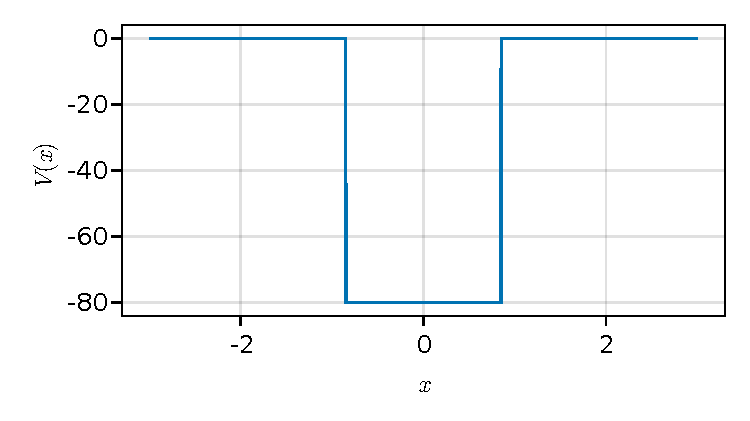
\includegraphics{jama.pdf}
    \caption{Potenciálová jáma.}
    \label{fig:potencial}
\end{figure}

\subsection*{Implementace}

Výpečet je prováděn na prostoru se součadnicí $x$ rodělenou na ${N}$ dílků. Proto je Hamiltonián reprezentován čtvercovou maticí ${N}\times{N}$ působící na $N$-rozměrný vektor $\ket{\Psi}$.

Laplaceův operátor je reprezentován maticí
 $$\Delta = \frac{1}{(\mathrm{d}x)^2}\left(\begin{matrix}
    -2  & 1 & 0  &\dots & 0 \\
    1  & -2& 1 & \dots& 0\\
    0 & 1   & -2&  \ddots & \vdots\\
    \vdots & \vdots   & \ddots & \ddots& 1\\
    0 & 0   & \dots & 1 & -2\\
\end{matrix}\right)$$
a celý Hamiltonián následně vypadá
$$ \hat{H} =  \frac{\hbar^2}{2m} \frac{1}{(\mathrm{d}x)^2}\left(\begin{matrix}
    -2  & 1 & 0  &\dots & 0 \\
    1  & -2& 1 & \dots& 0\\
    0 & 1   & -2&  \ddots & \vdots\\
    \vdots & \vdots   & \ddots & \ddots& 1\\
    0 & 0   & \dots & 1 & -2\\
\end{matrix}\right) + \mathrm{diag}(V(x)) $$
Řešení rovnice se redukuje na hledání vlastních hodnot a hlastních vektorů matice Hamiltoniánu.

\subsection*{Co mne na řešení zaujalo?}

Na řešení mne zaujalo, jak jednoduše proveditelné je. V podstatě jediné o co jde, je sestrojit matici a najít její vlastní čísla a vlastní vektory. Toto může velmi usnadnit řešení komplikovanějších úloh.

Výpočet byl implementován zároveň v Pythonu s užitím knihoven NumPy a v Julii. Pro porovnání byl proveden výpočet stejné jámy s $N = 6000$ v Pythonu a v Julii s využitím 32 a 64 bitových proměnných. Volba $N$ je volena tak, aby výpočet trval lehce přes minutu. Při řešení na notebooku vyšla nejrychleji Julia s 64 bitovou reprezentací. Ukázalo se, že kompilovaná Julie je rychlejší než Pythonovské knihovny a to zhruba dvakrát. To, že 64 bitový reprezentace je rychlejší, je pravděpodobně způsobeno procesorem, který je taktéž 64 bitový.

\begin{figure}
    \centering
    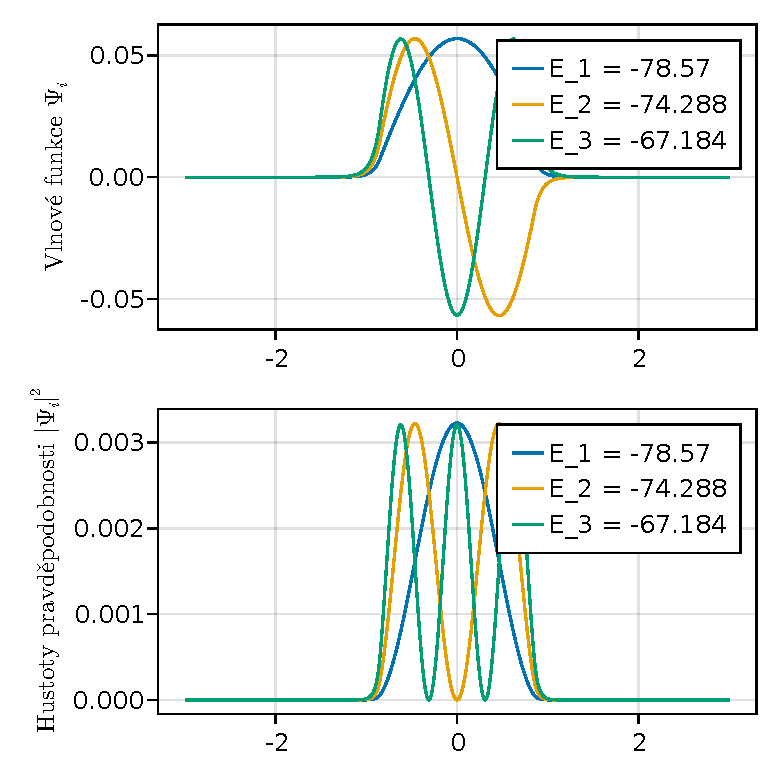
\includegraphics{figure.pdf}
    \caption{Výsledek výpočtu pro jámu šířky $d = 1,7$ a hloubky $L =80$. Vykreslené první tři stavy a příslušné hustoty pravděpodobnosti. Vykresleno pomocí knihovny Makie.}
    \label{fig:vysledek}
\end{figure}


\subsection*{Výsledky výpočtu}
Výsledky Lze visdět na obrázku \ref{fig:vysledek}, kde jsou vykresleny první tři stavy. Při provední výpočtu pro mělčí jámu (d = 15) lze vidět prosakování mimo jámu zvláště u vyšších energiových stavů. Výsledek lze vidět na obrázku \ref{fig:vysledek_1}.

\begin{figure}
    \centering
    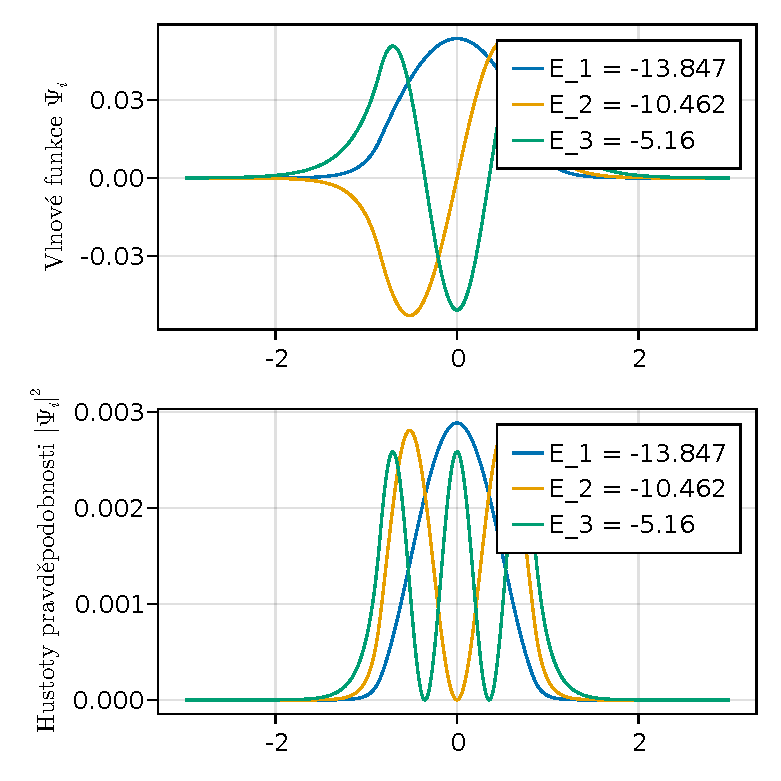
\includegraphics{figure_1.pdf}
    \caption{Výsledek výpočtu pro jámu šířky $d = 1,7$ a hloubky $L =20$. Vykreslené první tři stavy a příslušné hustoty pravděpodobnosti. Vykresleno pomocí knihovny Makie.}
    \label{fig:vysledek_1}
\end{figure}

\end{document}